%
\documentclass[11pt]{article}

\usepackage[left=3cm,top=2cm,bottom=2cm,right=3cm]{geometry}
\usepackage{amsmath}
\usepackage{amsfonts}
\usepackage{algorithm}
\usepackage{algorithmic}
\usepackage{array}
\usepackage{graphicx}
\usepackage{subfigure}
\usepackage{epsf}
\usepackage{psfrag}
\usepackage{epsfig}
\usepackage{textcomp}
\usepackage{hyperref}
\newcommand{\comment}[1]{{}}

\newcommand{\hwproblem}[2] {\noindent \\ {\bf #1} {\it #2}}

\newcommand{\textbox}[1]{\hfill\rule{0ex}{0.01ex}
 \centerline{\fbox{\parbox{\textwidth}{#1}}}}


\pagestyle{plain} % Header is clear and the footer contains the page number
\setlength{\parindent}{0pt}
\addtolength{\parskip}{\baselineskip}


\begin{document}


% Header
\begin{center}
\small{MIT CSAIL} \\
\vspace{0.1cm}
\large{6.8300/1 Advances in Computer Vision} \\
\vspace{0.2cm}
Spring 2024\\
\vspace{1cm}
{\bf Problem Set 1}
\vspace{0.2cm}
\end{center}

% Administration
\textbox{
\textbf{Posted:} Tuesday, February 13, 2024   \hfill  \textbf{Due:} Thursday 23:59, Feb 22, 2024\\
\\
6.8300/1 students are expected to finish all problems unless otherwise indicated. \\

The relevant material for this Problem Set was covered in Lectures 1 and 2.\\

\textbf{Attention: If you fail to include screenshots of your code in your report, we will not be able to give you points for your code, so please do not forget.}\\

We provide a Python notebook with the code to be completed. You can run it locally or on Google Colab. To use Colab, upload it to Google Drive and double-click the notebook (or right-click and select Open with Google Colaboratory),  which will allow you to complete the problems without setting up your own environment. Once you have  finished, copy the code sections that  you have completed\ as screenshots to the report. \\

Please submit (1) a report named \texttt{kerberos-id.pdf} including your answers to all required questions with images and/or plots showing your derivations/results and screenshots of the code you wrote. 
(2) There will also be a secondary Gradescope submission assignment pset 1b to upload your Python notebook, with the cells run and the relevant source code. We cannot dive into your code for grading (only for honor code violations), so missing code screenshots in the \texttt{.pdf} mean missing work.\\

Submission links will be released at least two days before the deadline; in the meantime we are getting section information in order.\\

 \textbf{Late Submission Policy:} If your pset is submitted within 7 days of the original deadline, you will receive partial credit. Such submissions will be penalized by a multiplicative coefficient that linearly decreases from 1 to 0.5 in discrete jumps.}\\
% \textbf{Late Submission Policy:} We do not accept late submissions. The submission deadline has a 50-minute soft cut-off; after midnight Thursday, submissions are penalized 2\% per minute late.\\}\\
\vspace{0.2cm}

\newpage

\hwproblem{Problem 1}{Perspective and orthographic projections} (10 points)

The goal of this first exercise is to take images with different settings of a camera to create pictures with perspective projection and with orthographic projection. Both pictures should cover the same piece of the scene. You can take pictures of real places or objects (e.g. your furniture), as long as there are some straight edges in the picture.% (e.g., the street, a living room, ...) or you can also create your own simple world (e.g., you can print \texttt{simpleWorld.pdf} and create your own scenes. I recommend printing on matte paper).

To create pictures with orthographic projection you can do two things: 1) use the zoom of the camera, 2) crop the central part of a picture. You will have to play with the distance between the camera and the scene, and with the zoom or cropping so that both images look as similar as possible, only differing in the type of projection (similar to the two images on slide 38 in the lecture 1 notes or in section 2.2 of the course notes (Figure 2.2)).

In some image editing tool (e.g. Google Slides or a pdf editor), find straight edges in the pictures and add red lines highlighting and extending those edges.

(1) Submit the two pictures and (2) add a sentence to describe the differences in their projection types with reference to your red lines.

\hwproblem{Problem 2}{Orthographic projection equations} (10 points)

Recall the parallel projection equations stated in class:
\begin{gather}
    x = \alpha  X + x_0\\
    y = \alpha (\cos(\theta)Y - \sin(\theta)Z) +y_{0}
\end{gather}
which relate the coordinates of a point in the 3D world to the image coordinates of an orthogonal camera rotated by $\theta$ over the $X$-axis (see book, Fig. 2.3).

Show that the  equations emerge naturally from a series of transformations
applied to the 3D world coordinates $(X,Y,Z)$, of the form:
\begin{gather}
\left[
  \begin{array}{c}
    x \\
    y
  \end{array}
\right] = \alpha \cdot P \cdot R_x(\theta) \cdot
\left[
  \begin{array}{ccc}
    X \\
    Y \\
    Z
  \end{array}
\right] +
\left[
  \begin{array}{c}
    x_0 \\
    y_0
  \end{array}
\right]
\end{gather}
Where $R_x(\theta)$ is a $3\times 3$ matrix corresponding to a rotation over the $X$ axis, $P$ is a $2 \times 3$ matrix corresponding to the orthogonal projection and $\alpha$ is  a scaling factor to account for the size
of the
camera sensor, which is a single scalar when the pixels are square (assumed in this case).  

Then, find $\alpha$, $x_0$ and $y_0$ when the world point $(0, 0, 0)$ projects onto  $(0, 0)$ \ (which corresponds to the center of the image) and the point $(1, 0, 0)$ projects onto $(3, 0)$.



\hwproblem{Problem 3}{Edge and surface constraints} (10 points)

In the lecture 1 slides, we have written down the constraints for $Y(x, y)$. Briefly derive the constraints for $Z(x, y)$ along vertical edges, horizontal edges, and flat surfaces.

\newpage
\hwproblem{Problem 4}{Complete the code} (20 points)

Fill in the missing lines (look for  \texttt{TODO}  comments) in the provided notebook \texttt{pset1.ipynb}, and include them in the report as screenshots. Also, include the generated plots in your report. First, find a way to classify edges as contact, vertical, or horizontal edges. Next, fill in the rest of the conditions of the constraint matrix. The constraints for when the pixel is on the ground have already been done for you as an example. Put the kernel in \texttt{Aij} and the value you expect in \texttt{b} (the conversion to a linear system is done for you later so you don't need to worry about that part). (\textit{Hint:} It may be helpful to refer to \href{https://en.wikipedia.org/wiki/Sobel_operator}{Sobel operators} and \href{https://en.wikipedia.org/wiki/Discrete_Laplace_operator}{discrete Laplace operators} to do this section).



\hwproblem{Problem 5}{Run the code} (10 points)

Rerun the script with at least two more of the provided images (e.g., \texttt{img2} and \texttt{img3}) and for each image try at least two different view angles. Include the generated plots in your report.

Optional: You can also try with new images taken by you if you decide to create your own simple world.

\hwproblem{Problem 6}{Violating simple world assumptions} (10 points)

Find one example from the four images provided with the problem set (\texttt{img1}, ..., \texttt{img4}) when the recovery of 3D information fails. Include the image and the reconstruction in your writeup, and explain why it fails.

\hwproblem{Problem 7}{Lenses} (20 points)

In class and the class notes, we derived the lensmaker's equation for the case of a symmetric thin lens, of radius of curvature $R$ for the front and back surfaces of the lens. Suppose, instead, that we have a ``plano-convex" lens, with the front surface shape with a radius of curvature $R$, as before, but with a flat back surface.

\begin{figure}[!htb]
  \centering
  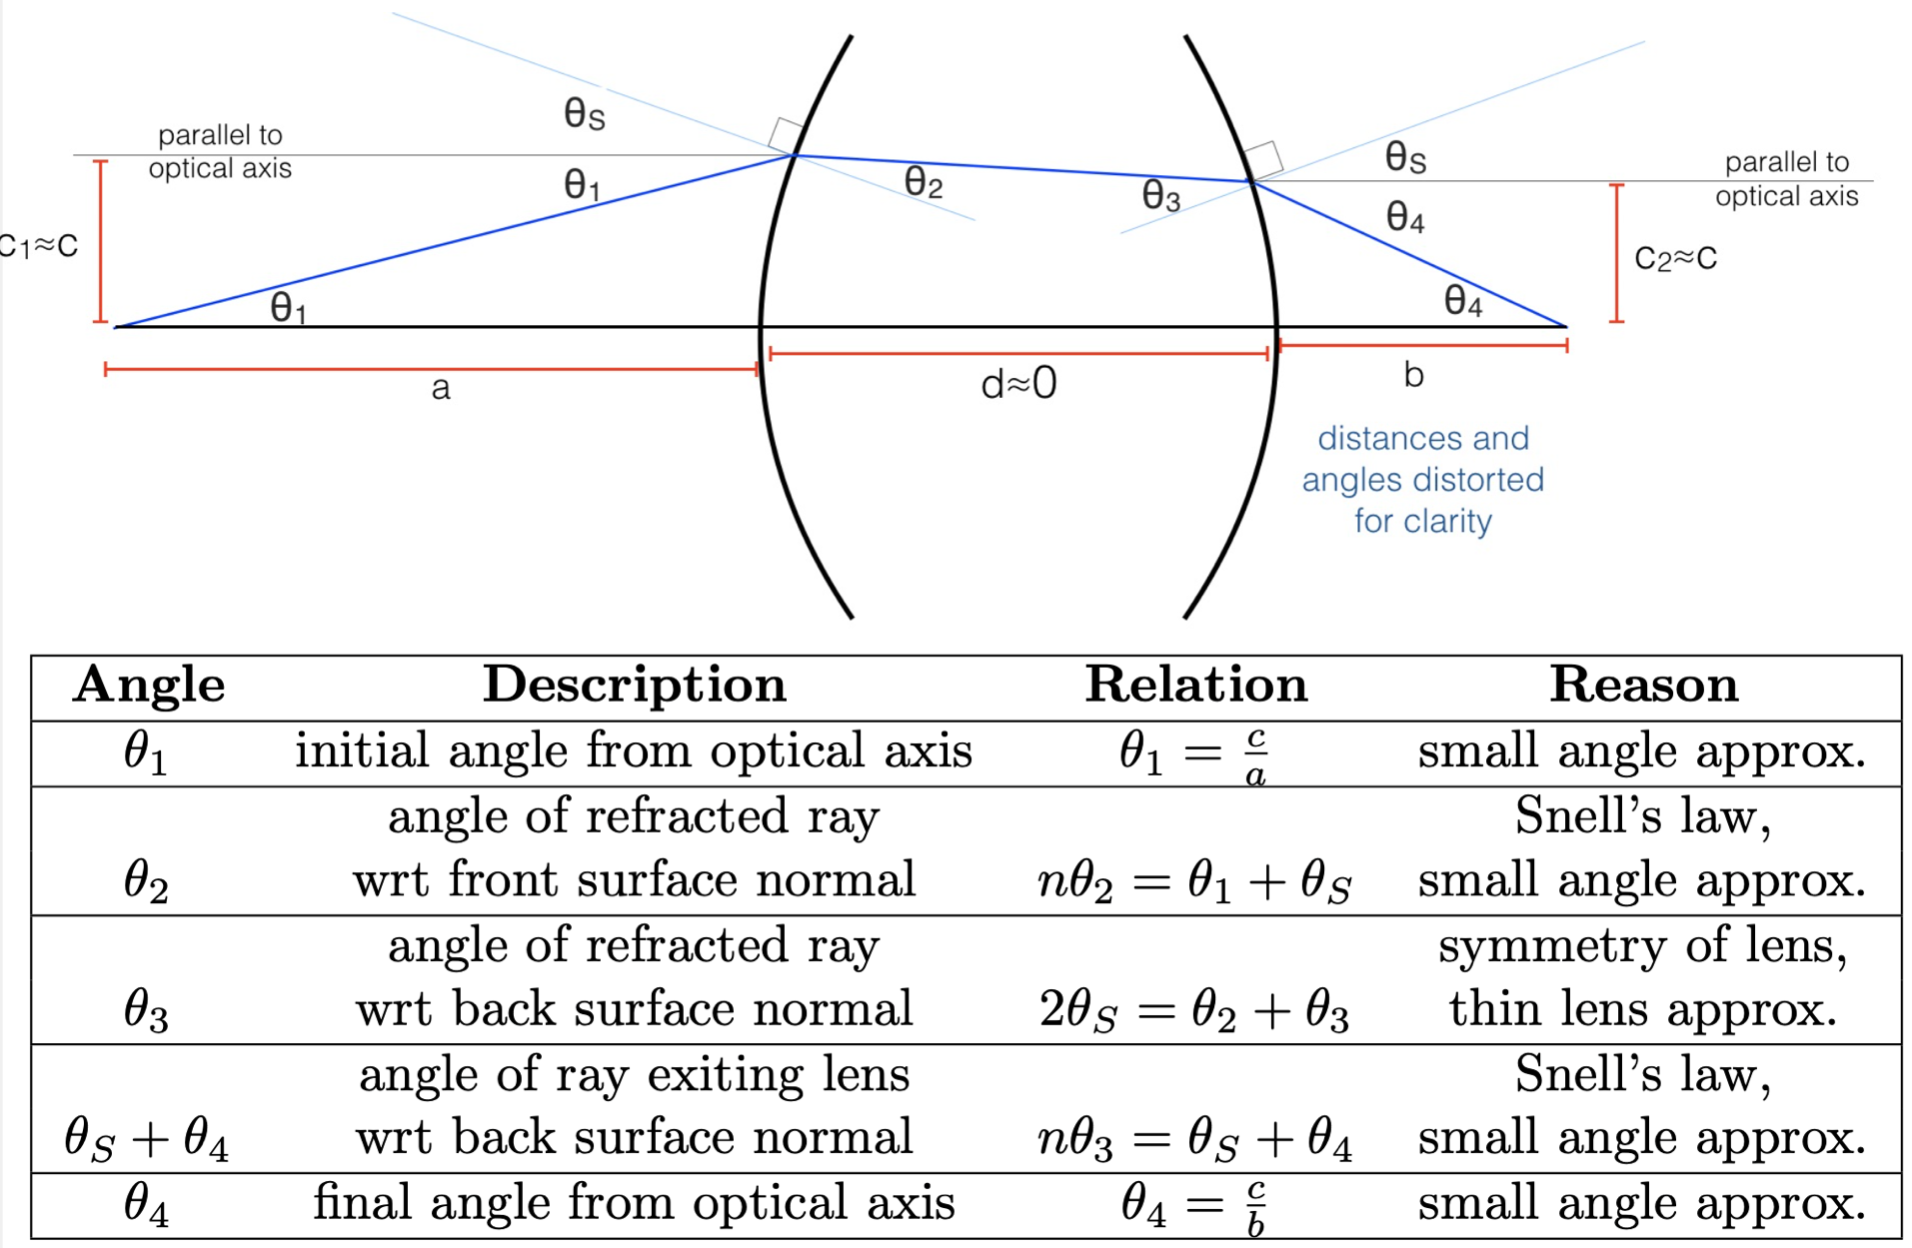
\includegraphics[width=.8\linewidth]{figures/fig_lens.png}
  \caption{Top: Diagram of a light ray passing through a symmetric thin lens. Bottom: Relations between angles of rays passing through the lens.}
  \label{fig_lens}
\end{figure}

\begin{figure}[!htb]
  \centering
  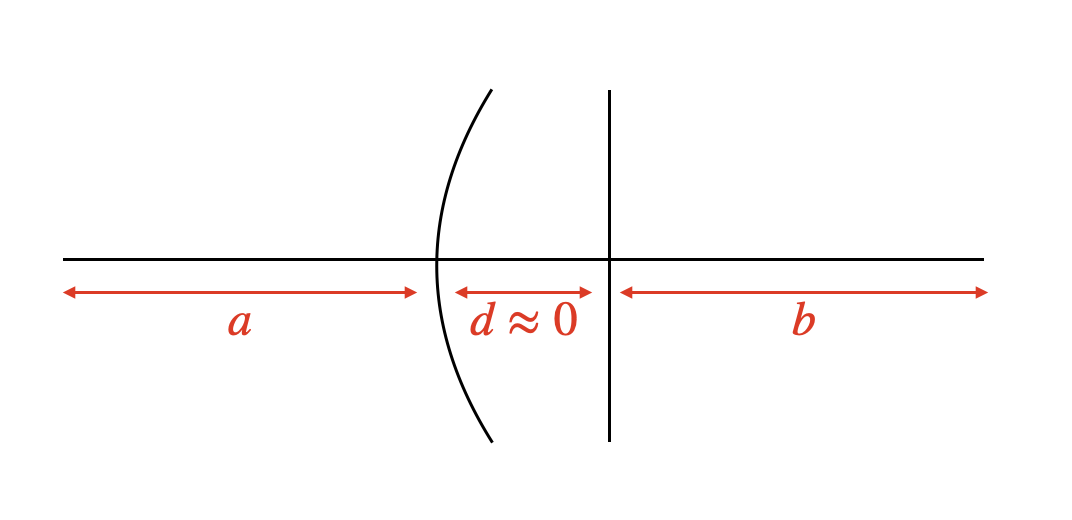
\includegraphics[width=.6\linewidth]{figures/fig_lens_plano_convex.png}
  \caption{Partial diagram of a plano-convex lens.}
  \label{fig_lens_planoconvex}
  \label{planoconv}
\end{figure}

(a) (1 point) Write down the 5 equations relating the angles of rays passing through a plano-convex lens. The symmetric lens case is shown in Figure \ref{fig_lens} (from Lecture 2 and Chapter 6 of the course notes). You may use the same variables and assumptions. A simplified diagram of the plano-convex lens is shown in Figure ~\ref{fig_lens_planoconvex}.

(b) (1 point) Using the equations from part (a) and the lensmaker's formula, find the expression for the lens focal length for the plano-convex lens described above, as shown in Fig.~\ref{planoconv}.

\hwproblem{Problem 8}{ Submit your \texttt{.ipynb} (fully run) at secondary Gradescope assignment.} (1 point)

\newpage
\hwproblem{Research problem} {The real world} [Optional]\\
Note: This problem is optional for all students, both graduate and undergraduate students. No credit will be given for this problem. It is just for fun!


\textit{A research problem is a question for which we do not know the answer. In fact, there might not
even be an answer. This question could be extended into a larger course project.}

The goal of this problem is to test the 3D reconstruction code with real images. A number of the assumptions we have made will not work when the input is real images of a more complex scene. For instance, the simple strategy of differentiating between foreground and background segmentation will not work with other scenes.

Try taking pictures of real-world scenes and propose modifications to the scheme proposed in this lecture so that you can get some better 3D reconstructions. The goal is not to build a general system, but to be able to handle a few more situations.
\end{document}
